%
% This file is automatically generated
%


%% meta-data %%

\documentclass[12pt]{article}
\usepackage{fullpage}
\usepackage{graphicx}
\usepackage{hyperref}
\usepackage{makecell}
\usepackage{multirow}
\usepackage{tabularx}
\usepackage{longtable}
\usepackage{caption}
\usepackage{wrapfig}

\renewcommand{\familydefault}{\sfdefault}

%% configuration %%

\title{Neo6502 Assembly - Messaging API}
\author{Paul Robson \\ Bill Auger}
\date{2024-03-01}

\graphicspath{ {./img/}                             % WRT local editor (eg: texworks)
               {./documents/release/source/img/}    % WRT command line
               {../documents/release/source/img/} } % WRT Makefile
\setcounter{tocdepth}{1}
\hypersetup{hidelinks , linktoc=all}


%% generic macros %%

% \MonoSp presents the given argument as a smaller mono-spaced font
\newcommand{\MonoSp}[1] {\fontsize{10pt}{10pt}\selectfont\texttt{#1}\normalsize}

% \Param presents the given argument as a "Param" in bold, mono-spaced font
\newcommand{\Param}[1] {\textbf{\texttt{Params[#1]}}}

% \ParamBits illustrates a bit-field
\newcommand{\ParamBits}[9] {
  \fontsize{10pt}{10pt}\selectfont
  \textbf{#1}
  \newline
  \begin{tabular}{ | c | c | c | c | c | c | c | c | }
    \hline
    bit-7 & bit-6 & bit-5 & bit-4 & bit-3 & bit-2 & bit-1 & bit-0 \\ \hline
    #2    & #3    & #4    & #5    & #6    & #7    & #8    & #9    \\ \hline
  \end{tabular}
  \normalsize
  \newline
}


%% special case macros %%

% \AddressCol expects to occupy a multicolumn(x2) column
% used in the "API Messaging Addresses" table, along with \BitsCol
\newcommand{\AddressCol}[1] { \multicolumn{2}{c|}{\MonoSp{#1}} }

% \BitsCol expects to occupy the second and third to last columns
% within a multirow(x8) row
% used in the "API Messaging Addresses" table, along with \AddressCol
\newcommand{\BitsCol}[9]{
    \multirow{8}{*}{\MonoSp{#1}} & \MonoSp{bit-7} & #2 \\ \cline{3-4}
  &                              & \MonoSp{bit-6} & #3 \\ \cline{3-4}
  &                              & \MonoSp{bit-5} & #4 \\ \cline{3-4}
  &                              & \MonoSp{bit-4} & #5 \\ \cline{3-4}
  &                              & \MonoSp{bit-3} & #6 \\ \cline{3-4}
  &                              & \MonoSp{bit-2} & #7 \\ \cline{3-4}
  &                              & \MonoSp{bit-1} & #8 \\ \cline{3-4}
  &                              & \MonoSp{bit-0} & #9 \\ \cline{3-4}
    \hline
}

% \ApiFnRow could technically work anyplace,
% but is mainly relevant for the API Functions table
\newcommand{\ApiFnRow}[3] {
  \makecell[tc]{#1 \\ #2}                                      &
  \makecell[tl]{\MonoSp{LDA \#\$0#1} \\ \MonoSp{STA \#\$FF01}} &
  #3                                                           \\ \hline
}

% \ParamsBytes could technically work anyplace,
% but is specifically for illustrating the Parameters to an API Function
\newcommand{\ParamsBytes}[9] {
  \fontsize{10pt}{10pt}\selectfont
  \textbf{#1}
  \newline
    \begin{tabular}{ | c | c | c | c | c | c | c | c | }                       \hline
      P0 & P1 & P2 & P3 & P4 & P5 & P6 & P7                                 \\
      \hline
      \MonoSp{\$FF04} & \MonoSp{\$FF05} & \MonoSp{\$FF06} & \MonoSp{\$FF07} &
      \MonoSp{\$FF08} & \MonoSp{\$FF09} & \MonoSp{\$FF0A} & \MonoSp{\$FF0B} \\ \hline
      \MonoSp{#2}     & \MonoSp{#3}     & \MonoSp{#4}     & \MonoSp{#5}     &
      \MonoSp{#6}     & \MonoSp{#7}     & \MonoSp{#8}     & \MonoSp{#9}     \\ \hline
    \end{tabular}
  \normalsize
  \newline
}

% \SpriteParamBits could technically work anyplace,
% but is specialized to illustrate the Sprite bit-field layout
\newcommand{\SpriteParamBits}[4] {
  \fontsize{10pt}{10pt}\selectfont
  \textbf{#1}
  \newline
  \begin{tabular}{ | c | c | c | c | c | c | c | c | }                    \hline
    \MonoSp{bit-7} & \MonoSp{bit-6} & \MonoSp{bit-5} & \MonoSp{bit-4}  &
    \MonoSp{bit-3} & \MonoSp{bit-2} & \MonoSp{bit-1} & \MonoSp{bit-0}  \\ \hline
    \MonoSp{#2}    & \MonoSp{#3}    & \multicolumn{6}{c|}{\MonoSp{#4}} \\ \hline
  \end{tabular}
  \normalsize
  \newline
}


%% document body %%

\begin{document}

\maketitle

\begin{center}
  
\includegraphics[scale=2.0]{neo6502-text-logo.png}
\end{center}

\tableofcontents


\pagebreak


\section{Neo6502 Messaging API}\label{api}

The Neo6502 API is a messaging system.
There are no methods to access the hardware directly.
Messages are passed via the block of memory from \MonoSp{\$FF00} to \MonoSp{\$FF0F},
as specified in the "API Messaging Addresses" table on the following page.
\newline

The kernel include file \MonoSp{documents/release/neo6502.inc}
specifies the beginning of this address range as the identifier \MonoSp{ControlPort},
along with the addresses of \MonoSp{WaitMessage} and \MonoSp{SendMessage} (described later),
various related kernel jump vectors, and some helper functions.
\newline

The application include files \MonoSp{examples/assembly/neo6502.asm.inc}
and \MonoSp{examples/C/neo6502.h}
also specify the beginning of this address range as the identifier \MonoSp{ControlPort}.
The assembly include also specifies \MonoSp{ControlPort} and the other controls as
\MonoSp{API\_COMMAND}, \MonoSp{API\_FUNCTION}, \MonoSp{API\_ERROR},
\MonoSp{API\_STATUS}, and \MonoSp{API\_PARAMETERS}.
The C header also specifies \MonoSp{ControlPort} and the other controls as
\MonoSp{API\_COMMAND\_ADDR}, \MonoSp{API\_FUNCTION\_ADDR},
\MonoSp{API\_ERROR\_ADDR}, \MonoSp{API\_STATUS\_ADDR},
and \MonoSp{API\_PARAMETERS\_ADDR}.
\newline

API Commands/Functions are grouped by functionality.
For example, Group 1 are system-related, and Group 2 are console-I/O-related.
All Groups and their Commands/Functions are shown in the following table.
\newline

Command/Function Parameters are notated in this document as \Param{0} through \Param{7},
or as a list or range (eg: \Param{1,2}, \Param{0..7}).
Note that these are referring to a mapping to memory locations.
The numbers represent offsets from the Parameters base address \MonoSp{\$FF04}.
Ie: the actual bytes are not necessarily all distinct "parameters" in the conventional sense.
Depending on the routine, a logical parameter may be an individual byte,
one or more bits of a byte interpreted as a composite or bit-field,
or multiple adjacent bytes interpreted as 16 or 32 bit values.
For example, the list \Param{0,1} would indicate a single logical parameter,
comprised of the two adjacent bytes \MonoSp{\$FF04} and \MonoSp{\$FF05}.
The range \Param{4..7} would indicate a single logical parameter,
spanning consecutive bytes between \MonoSp{\$FF08} and \MonoSp{\$FF0B}.
\newline

\textbf{Note that strings referenced by Parameters are not ASCIIZ, but are length-prefixed.}
The first byte represents the length of the string (not counting itself). The string begins at the second byte.
Consequently, strings must be 256 bytes or less (not counting the length header).
\newline


\pagebreak


\begin{table}[h]
\centering\textbf{API Messaging Addresses} \\
\begin{tabularx}{1\textwidth}{|>{\centering\arraybackslash}m{0.150\textwidth}|
                               >{\centering\arraybackslash}m{0.075\textwidth}|
                               >{\centering\arraybackslash}m{0.075\textwidth}|
                               >{\arraybackslash}m{0.594\textwidth}|}
  \hline
  \textbf{Meta} & \AddressCol{Address} & \textbf{Contents}
  \\ \hline
  Group & \AddressCol{\MonoSp{\$FF00}} &
  Group selector and status.
  Writing a non-zero value to this location triggers the routine specified in \MonoSp{\$FF01}.
  The system will respond by setting the 'Error', 'Information', and 'Parameters'
  values appropriately.
  Upon completion, this memory location will be will cleared.
  \\ \hline
  Function & \AddressCol{\$FF01} &
  A command or function within the selected Group.
  For example, Group 1 Function 0 writes a value to the console;
  and Group 1 Function 1 reads the keyboard.
  \\ \hline
  Error & \AddressCol{\$FF02} &
  Return any error values, 0 = no error.
  \\ \hline
  \multirow{8}{*}{Information} &
  \BitsCol{\$FF03}{                                                    % address
  Set (\MonoSp{1}) if the ESCape key has been pressed.                 % desc of bit0
  This is not automatically reset.                                     % desc of bit0
  }{\textit{unused}}{\textit{unused}}{\textit{unused}}                 % desc of bits1..3
  {\textit{unused}}{\textit{unused}}{\textit{unused}}{\textit{unused}} % desc of bits4..7
  Parameters & \AddressCol{\$FF04..B} &
  This memory block is notated in this document as \Param{0} through \Param{7},
  or as a composite list or range (eg: \Param{1,2}, \Param{0..7}).
  Some Functions require Parameters in these locations
  and some return values in these locations; yet others do neither.
  \\ \hline
  Reserved & \AddressCol{\$FF0C..F} &
  Reserved.
  \\ \hline
\end{tabularx}
\end{table}


\pagebreak


\subsection{API Interfacing Protocol}\label{subsec:api-protocol}

Neo6502 application programmers should interact with the API
per the following algorithm:

\begin{enumerate}
  \item Wait for any pending command to complete.
        There is a subroutine \MonoSp{WaitMessage} which does this for the developer.
  \item Setup the Function code at \MonoSp{\$FF01};
        and any Parameters across \MonoSp{\$FF04..\$FF0B}.
        To print a character for example, set \MonoSp{\$FF01} to \MonoSp{\$06}
        and set \MonoSp{\$FF04} to the character's ASCII value.
        To draw a line, set \MonoSp{\$FF01} to \MonoSp{\$02}
        and set \MonoSp{\$FF04..\$FF0B} as four 16-bit pixel coordinates:

        \ParamsBytes{Params}{srcX lo}{srcX hi}{srcY lo}{srcY hi}{destX lo}{destX hi}{destY lo}{destY hi}
  \item Setup the command code at \MonoSp{\$FF00}. This triggers the routine;
        so mind that the Function code and Parameters are setup sanely prior.
        On a technical point, both implementations process the message immediately on write.
% Q2: both implementations of what?
%     eg: "... both the _?_ and the _?_ implementation process the message immediately ..."
  \item Optionally, wait for completion.
        Most commands (eg: writing to the console) do not require waiting,
        as any subsequent command will wait/queue as per step 1.
        Query commands (e.g. reading from the keyboard queue),
        return a value in a parameter.
        Programs must wait until the control address \MonoSp{\$FF00} has been cleared
        before reading the result of a query.
\end{enumerate}

There is a support function \MonoSp{SendMessage},
which in-lines the command and function.
E.g.: this code from the Kernel:

% Q1: KSendMessage/KWaitMessage or SendMessage/WaitMessage ?
\begin{verbatim}
jsr KSendMessage ; send message for command 2,1 (read keyboard)
.byte 2,1
jsr KWaitMessage ; wait to receive the result message
lda DParameters  ; read result
\end{verbatim}

The instructions above are equivalent to the following explicit steps:
\begin{verbatim}
lda #1
sta DFunction
lda #2
sta DCommand    ; trigger API function 2,1 (read keyboard)
Loop:
lda DCommand    ; load the result - non-zero until the routine's completion
bne Loop        ; wait for API routine to complete
lda DParameters ; read result (a key-code)
\end{verbatim}


\pagebreak


\section{API Functions}\label{api-functions}

The following tables are a comprehensive list of all supported API functions.
\newline

For the convenience of application programmers,
the application include files \MonoSp{examples/C/neo6502.h}
and \MonoSp{examples/assembly/neo6502.asm.inc}
define macros for these groups, their functions,
and common parameters (colors, musical notes, etc).


% makedispatch: BEGIN
\begin{longtable*}{ | c | l | p{12cm} | }
\caption*{Group 1 - System Functions} \\
\hline
\textbf{Function} & \textbf{Assembly} & \textbf{Description} \\
\hline
\endfirsthead
\caption*{Group 1 - System Functions (continued)} \\
\hline
\textbf{Function} & \textbf{Assembly} & \textbf{Description} \\
\hline
\endhead
\ApiFnRow{0}{Reset}{
Resets the messaging system and component systems.
Normally, should not be used.
}
\ApiFnRow{1}{Timer}{
Deposit the value (32-bits) of the 100Hz system timer into \Param{0..3}.
}
\ApiFnRow{2}{Key Status}{
Deposit the state of the specified keyboard key into \Param{0}.
The key which to query is specified in \Param{0}.
}
\ApiFnRow{3}{Basic}{
Loads and allows the execution of BASIC via a indirect jump through address zero.
}
\ApiFnRow{4}{Credits}{
Print the Neo6502 project contributors (stored in flash memory).
}
\ApiFnRow{5}{Serial Status}{
Check the serial port to see if there is a data transmission.
}
\ApiFnRow{6}{Locale}{
Set the locale code specified in \Param{0,1} as upper-case ASCII letters.
\Param{0} takes the first letter and \Param{1} takes the second letter.
For example:
\begin{description}
\item English:\MonoSp{~\Param{0}\textless-\$45} ('E') and \MonoSp{\Param{1}\textless-\$4E} ('N')
\item French:\MonoSp{~~\Param{0}\textless-\$46} ('F') and \MonoSp{\Param{1}\textless-\$52} ('R')
\end{description}
}
\ApiFnRow{7}{System Reset}{
System Reset. This is a full hardware reset. It resets the RP2040 using the Watchdog timer, and
this also resets the 65C02.
}
\end{longtable*}
\pagebreak
\begin{longtable*}{ | c | l | p{12cm} | }
\caption*{Group 2 - Console Functions} \\
\hline
\textbf{Function} & \textbf{Assembly} & \textbf{Description} \\
\hline
\endfirsthead
\caption*{Group 2 - Console Functions (continued)} \\
\hline
\textbf{Function} & \textbf{Assembly} & \textbf{Description} \\
\hline
\endhead
\ApiFnRow{0}{Write Character}{
Function 0 is console out (duplicate of Function 6 for backward compatibility).
}
\ApiFnRow{1}{Read Character}{
Read and remove a key press from the keyboard queue into \Param{0}.
This is the ASCII value of the keystroke.
If there are no key presses in the queue, \Param{0} will be zero.
\newline

Note that this Function is best for text input, but not for games.
Function 7,1 is more optimal for games, as this only detects key presses,
you cannot check whether the key is currently down or not.
}
\ApiFnRow{2}{Console Status}{
Check to see if the keyboard queue is empty.
If it is, \Param{0} will be \MonoSp{\$FF}, otherwise it will be \MonoSp{\$00}.
}
\ApiFnRow{3}{Read Line}{
Input the current line below the cursor into \Param{0,1} as a length-prefixed string;
and move the cursor to the line below. Handles multiple-line input.
}
\ApiFnRow{4}{Define Hotkey}{
Define the function key F1..F10 (\MonoSp{\$01..\$0A}) specified in \Param{0} to emit the
length-prefixed string stored at the memory location specified in \Param{2,3}.
For example, in a block of in-line assembly within a BASIC program,
the string: \MonoSp{06,12,108,105,115,116,13} would clear the screen (\MonoSp{12}),
then list the program (\MonoSp{108}='l',\MonoSp{105}='i',\MonoSp{115}='s',\MonoSp{116}='t',\MonoSp{13}='ENTER').
\newline F11 and F12 cannot currently be defined.
}
\ApiFnRow{5}{Define Character}{
Define a font character specified in \Param{0} within the range of 192..255.
Fill bits 0..5 (columns) of \Param{1..7} (rows) with the character bitmap.
}
\ApiFnRow{6}{Write Character}{
Write the character specified in \Param{0} to the console at the cursor position.
Refer to Section \#\ref{console-codes} "Console Codes" for details.
}
\ApiFnRow{7}{Set Cursor Pos}{
Move the cursor to the screen character cell \Param{0}\textless-X, \Param{1}\textless-Y.
}
\ApiFnRow{8}{List Hotkeys}{
Display the current function key definitions.
}
\ApiFnRow{9}{Screen Size}{
Fetches the console size, in characters, to \Param{0} and \Param{1}, the height and width respectively.
}
\ApiFnRow{10}{Insert Line}{
Insert Line
This is a support function which inserts a blank line in the console and should not be used.
}
\ApiFnRow{11}{Delete Line}{
Delete Line
This is a support function which deletes a line in the console and should not be used.
}
\ApiFnRow{12}{Clear Screen}{
Clears the screen.
}
\ApiFnRow{13}{Cursor Position}{
Get Cursor Position
\newline Returns the current cursor position in \Param{0} and \Param{1}
}
\ApiFnRow{14}{Clear Region}{
Erase all characters within the rectangular region specified
in \Param{0,1} (begin X,Y) and \Param{2,3} (end X,Y).
}
\ApiFnRow{15}{Set Text Color}{
Set Text Color
\newline Sets the foreground colour to \Param{0} and the background colour to \Param{1}
}
\ApiFnRow{16}{Cursor Inverse}{
Toggles the cursor colour between normal and inverse
(ie: swaps FG and BG colors). This should not be used.
}
\end{longtable*}
\pagebreak
\begin{longtable*}{ | c | l | p{12cm} | }
\caption*{Group 3 - File I/O Functions} \\
\hline
\textbf{Function} & \textbf{Assembly} & \textbf{Description} \\
\hline
\endfirsthead
\caption*{Group 3 - File I/O Functions (continued)} \\
\hline
\textbf{Function} & \textbf{Assembly} & \textbf{Description} \\
\hline
\endhead
\ApiFnRow{1}{List Directory}{
Display the file listing of the present directory.
}
\ApiFnRow{2}{Load File}{
Load a file by name into memory. On input:
\begin{itemize}
\item \Param{0,1} points to the length-prefixed filename string;
\item \Param{2,3} contains the location to write the data to. If the
address is \MonoSp{\$FFFF}, the file will instead be loaded into the
graphics working memory, used for sprites, tiles, images.
\end{itemize}
On output:
\begin{itemize}
\item \Param{0} contains an error/status code.
\end{itemize}
}
\ApiFnRow{3}{Store File}{
Saves data in memory to a file. On input:
\begin{itemize}
\item \Param{0,1} points to the length-prefixed filename string;
\item \Param{2,3} contains the location to read data from;
\item \Param{4,5} specified the number of bytes to styore.
\end{itemize}
On output:
\begin{itemize}
\item \Param{0} contains an error/status code.
\end{itemize}
}
\ApiFnRow{4}{File Open}{
Opens a file into a specific channel. On input:
\begin{itemize}
\item \Param{0} contains the file channel to open;
\item \Param{1,2} contains the length-prefixed filename;
\item \Param{3} contains the open mode. See below.
\end{itemize}
Valid open modes are:
\begin{itemize}
\item 0 opens the file for read-only access;
\item 1 opens the file for write-only access;
\item 2 opens the file for read-write access;
\item 3 creates the file if it doesn't already exist, truncates it if it
does, and opens the file for read-write access.
\end{itemize}
Modes 0 to 2 will fail if the file does not already exist. If the
channel is already open, the call fails. Opening the same file more than
once on different channels has undefined behaviour and is not
recommended.
}
\ApiFnRow{5}{File Close}{
Closes a particular channel. On input:
\begin{itemize}
\item \Param{0} contains the file channel to close.
\end{itemize}
}
\ApiFnRow{6}{File Seek}{
Seeks the file opened on a particular channel to a location. On input:
\begin{itemize}
\item \Param{0} contains the file channel to operate on;
\item \Param{1,2,3,4} contains the file location.
\end{itemize}
You can seek beyond the end of a file to extend the file. Whether the
file size changes when the seek happens or when you perform the write is
undefined.
}
\ApiFnRow{7}{File Tell}{
Returns the current seek location for the file opened on a particular channel. On input:
\begin{itemize}
\item \Param{0} contains the file channel to operate on.
\end{itemize}
On output:
\begin{itemize}
\item \Param{1,2,3,4} contains the file location.
\end{itemize}
}
\ApiFnRow{8}{File Read}{
Reads data from an opened file. On input:
\begin{itemize}
\item \Param{0} contains the file channel to operate on;
\item \Param{1,2} points to the destination in memory, or \MonoSp{\$FFFF}
to write to graphics memory;
\item \Param{2,3} contains the amount of data to read.
\end{itemize}
On output:
\begin{itemize}
\item \Param{2,3} is updated to contain the amount of data actually read.
\end{itemize}
Data is read from the current seek position, which is advanced after the
read.
}
\ApiFnRow{9}{File Write}{
Writes data to an opened file. On input:
\begin{itemize}
\item \Param{0} contains the file channel to operate on;
\item \Param{1,2} points to the data in memory;
\item \Param{2,3} contains the amount of data to write.
\end{itemize}
On output:
\begin{itemize}
\item \Param{2,3} is updated to contain the amount of data actually written.
\end{itemize}
Data is written to the current seek position, which is advanced after the
write.
}
\ApiFnRow{10}{File Size}{
Returns the current size of an opened file. On input:
\begin{itemize}
\item \Param{0} contains the file channel to operate on.
\end{itemize}
On output:
\begin{itemize}
\item \Param{1,2,3,4} contains the size of the file.
\end{itemize}
This call should be used on open files and takes into account any
buffered data which has not yet been written to disk. As a result it may
return a different size to the stat API call described below.
}
\ApiFnRow{11}{File Set Size}{
Extends or truncates an opened file to a particular size. On input:
\begin{itemize}
\item \Param{0} contains the file channel to operate on;
\item \Param{1,2,3,4} contains the new size of the file.
\end{itemize}
}
\ApiFnRow{12}{File Rename}{
Renames a file. On input:
\begin{itemize}
\item \Param{0,1} points to the length-prefixed string for the old name;
\item \Param{2,3} points to the length-prefixed string for the new name.
\end{itemize}
Files may be renamed across directories.
}
\ApiFnRow{13}{Delete File}{
Deletes a file or directory. On input:
\begin{itemize}
\item \Param{0,1} points to the length-prefixed filename string.
\end{itemize}
Deleting a file which is open has undefined behaviour. Directories may
only be deleted if they are empty.
}
\ApiFnRow{14}{Create Directory}{
Creates a new directory. On input:
\begin{itemize}
\item \Param{0,1} points to the length-prefixed filename string.
\end{itemize}
}
\ApiFnRow{15}{Change Directory}{
Changes the current working directory. On input:
\begin{itemize}
\item \Param{0,1} points to the length-prefixed path string.
\end{itemize}
}
\ApiFnRow{16}{Stat File}{
Retrieves information about a file by name. On input:
\begin{itemize}
\item \Param{0,1} points to the length-prefixed filename string.
\end{itemize}
On output:
\begin{itemize}
\item \Param{0,1,2,3} contains the length of the file;
\item \Param{4} contains the attribute bitfield of the file.
\end{itemize}
If the file is open for writing, this may not return the correct size
due to buffered data not having been flushed to disk.
File attributes are a bitfield as follows:
\newline

\ParamBits{File attributes}
{0}
{0}
{0}
{Hidden}
{Read only}
{Archive}
{System}
{Directory}
}
\ApiFnRow{17}{Open Directory}{
Opens a directory for enumeration. On input:
\begin{itemize}
\item \Param{0,1} points to the length-prefixed filename string.
\end{itemize}
Only one directory at a time may be opened. If a directory is already
open when this call is made, it is automatically closed; however, an
open directory may make it impossible to delete the directory, so
closing the directory after use is good practice.
}
\ApiFnRow{18}{Read Directory}{
Reads an item from the currently open directory. On input:
\begin{itemize}
\item \Param{0,1} points to a length-prefixed buffer for returning the filename.
\end{itemize}
\begin{itemize}
\item \Param{0,1} is unchanged, but the buffer is updated to contain the
length-prefixed filename (without any leading path);
\item \Param{2,3,4,5} contains the length of the file;
\item \Param{6} contains the file attributes, as described by the Stat File call.
\end{itemize}
This call fails if there are no more items to read.
}
\ApiFnRow{19}{Close Directory}{
Closes any directory opened by Open Directory.
}
\ApiFnRow{20}{Copy File}{
Copies a file. On input:
\begin{itemize}
\item \Param{0,1} points to the length-prefixed old filename;
\item \Param{2,3} points to the length-prefixed new filename.
\end{itemize}
Only single files may be copied, not directories.
}
\ApiFnRow{32}{List Filtered}{
Prints a filtered file listing of the current directory to the console. On input:
\begin{itemize}
\item \Param{0,1} points to the filename search string.
\end{itemize}
Files will only be shown if the name contains the search string (via a
substring match).
}
\end{longtable*}
\pagebreak
\begin{longtable*}{ | c | l | p{12cm} | }
\caption*{Group 4 - Mathematics Functions} \\
\hline
\textbf{Function} & \textbf{Assembly} & \textbf{Description} \\
\hline
\endfirsthead
\caption*{Group 4 - Mathematics Functions (continued)} \\
\hline
\textbf{Function} & \textbf{Assembly} & \textbf{Description} \\
\hline
\endhead
\ApiFnRow{0}{Addition}{
Addition
\newline Register1 := Register 1 + Register2
}
\ApiFnRow{1}{Subtraction}{
Subtraction
\newline Register1 := Register 1 - Register2
}
\ApiFnRow{2}{Multiplication}{
Multiplication
\newline Register1 := Register 1 * Register2
}
\ApiFnRow{3}{Decimal Division}{
Decimal Division
\newline Register1 := Register 1 / Register2 (floating point)
}
\ApiFnRow{4}{Integer Division}{
Integer Division
\newline Register1 := Register 1 / Register2 (integer result)
}
\ApiFnRow{5}{Integer Modulus}{
Integer Modulus
\newline Register1 := Register 1 mod Register2
}
\ApiFnRow{6}{Compare}{
Compare Numbers
\newline \Param{0} := Register 1 compare Register2 : returns \$FF, 0, 1 for less equal and greater
\newline Note: float comparison is approximate because of rounding.
}
\ApiFnRow{16}{Negate}{
Negate
\newline Register1 :=  -Register 1
}
\ApiFnRow{17}{Floor}{
Floor
\newline Register1 := floor(Register 1)
}
\ApiFnRow{18}{Square Root}{
Square Root
\newline Register1 := square root(Register 1)
}
\ApiFnRow{19}{Sine}{
Sine
\newline Register1 := sine(Register 1) angles in degrees
}
\ApiFnRow{20}{Cosine}{
Cosine
\newline Register1 := cosine(Register 1) angles in degrees
}
\ApiFnRow{21}{Tangent}{
Tangent
\newline Register1 := tangent(Register 1) angles in degrees
}
\ApiFnRow{22}{Arctangent}{
Arctangent
\newline Register1 := arctangent(Register 1) angles in degrees
}
\ApiFnRow{23}{Exponent}{
Exponent
\newline Register1 :=  e to the power of Register 1
}
\ApiFnRow{24}{Logarithm}{
Logarithm
\newline Register1 := log(Register 1) natural logarithm
}
\ApiFnRow{25}{Absolute Value}{
Absolute Value
\newline Register1 := absolute value(Register 1)
}
\ApiFnRow{26}{Sign}{
Sign
\newline Register1 := sign(Register 1), returns -1 0 or 1
}
\ApiFnRow{27}{Random Decimal}{
Random Decimal
\newline Register1 := random float from 0-1
}
\ApiFnRow{28}{Random Integer}{
Random Integer
\newline Register1 := random integer from 0 to (Register 1-1)
}
\ApiFnRow{32}{Number to Decimal}{
Number to Decimal
\newline Helper function for tokeniser, do not use.
}
\ApiFnRow{33}{String to Number}{
String to Number
\newline Convert the length prefixed string at \Param{4,5} to a constant in Register1.
}
\ApiFnRow{34}{Number to String}{
Number to String
\newline TODO: Convert the constant in Register1 to a length prefixed string which is stored at \Param{4,5}
}
\end{longtable*}
\pagebreak
\begin{longtable*}{ | c | l | p{12cm} | }
\caption*{Group 5 - Graphics Functions} \\
\hline
\textbf{Function} & \textbf{Assembly} & \textbf{Description} \\
\hline
\endfirsthead
\caption*{Group 5 - Graphics Functions (continued)} \\
\hline
\textbf{Function} & \textbf{Assembly} & \textbf{Description} \\
\hline
\endhead
\ApiFnRow{1}{Set Defaults}{
Configure the global graphics system settings.
Not all parameters are relevant for all graphics commands;
but all parameters will be set by this command. So mind their values.
Refer to Section \#\ref{subsec:graphics-settings} "Graphics Settings" for details.
\newline

\ParamsBytes{Graphics Settings}{AND}{XOR}{Fill}{Extent}
{Flip}{unused}{\textit{unused}}{\textit{unused}}
\newline

\ParamBits{\$FF08 - Flip Axis Flags}{0}{0}{0}{0}{0}{0}{Vertical}{Horizontal}
}
\ApiFnRow{2}{Draw Line}{
Draw a line between the screen coordinates specified
in  \Param{0,1},\Param{2,3} (begin X,Y)
and \Param{4,5},\Param{6,7} (end X,Y).
\newline

\ParamsBytes{Draw Line Parameters}{X  lo}{X  hi}{Y  lo}{Y  hi}
{X' lo}{X' hi}{Y' lo}{Y' hi}
}
\ApiFnRow{3}{Draw Rectangle}{
Draw a rectangle spanning the screen coordinates specified
in  \Param{0,1},\Param{2,3} (corner X,Y)
and \Param{4,5},\Param{6,7} (opposite corner X,Y).
}
\ApiFnRow{4}{Draw Ellipse}{
Draw an ellipse spanning the screen coordinates specified
in  \Param{0,1},\Param{2,3} (corner  X,Y)
and \Param{4,5},\Param{6,7} (opposite corner X,Y).
}
\ApiFnRow{5}{Draw Pixel}{
Draw a single pixel at the screen coordinates specified
in \Param{0,1},\Param{2,3} (X,Y).
}
\ApiFnRow{6}{Draw Text}{
Draw the length-prefixed string of text stored
at the memory location specified in \Param{4,5}
at the screen character cell specified in \Param{0,1},\Param{2,3} (X,Y).
}
\ApiFnRow{7}{Draw Image}{
Draw the image with image ID in \Param{4}
at the screen coordinates \Param{0,1},\Param{2,3} (X,Y).
The extent and flip settings influence this command.
}
\ApiFnRow{8}{Draw Tilemap}{
Draw the current tilemap at the screen coordinates specified
in \Param{0,1},\Param{2,3} (top-left X,Y)
and \Param{4,5},\Param{6,7} (bottom-right X,Y)
using current graphics settings.
}
\ApiFnRow{32}{Set Palette}{
Set the palette colour at the index spcified in \Param{0}
to the values in \Param{1},\Param{2},\Param{3} (RGB).
}
\ApiFnRow{33}{Read Pixel}{
Read a single pixel at the screen coordinates specified
in \Param{0,1},\Param{2,3} (X,Y).
When the routine completes, the result will be in \Param{0}. If sprites are in use, this will be the
background only (0..15), if sprites are not in use it may return (0..255)
}
\ApiFnRow{34}{Reset Palette}{
Reset the palette to the defaults.
}
\ApiFnRow{35}{Set Tilemap}{
Set the current tilemap.
\Param{0,1} is the memory address of the tilemap,
and \Param{2,3},\Param{4,5} (X,Y) specifies the offset into the tilemap,
in units of pixels, of the top-left pixel of the tile.
}
\ApiFnRow{36}{Read Sprite Pixel}{
Read Pixel from the sprite layer at the screen coordinates
specified in \Param{0,1},\Param{2,3} (X,Y).
When the routine completes, the result will be in \Param{0}.
Refer to Section \#\ref{graphics-colors} "Pixel Colors" for details.
}
\ApiFnRow{37}{Frame Count}{
Deposit into \Param{0..3},
the number of v-blanks (full screen redraws) which have occurred since power-on.
This is updated at the start of each v-blank period.
}
\ApiFnRow{64}{Set Color}{
Set Color
\newline Sets the current drawing colour to \Param{0}
}
\ApiFnRow{65}{Set Solid Flag}{
Set Solid Flag
\newline Sets the solid flag to \Param{0}, which indicates either solid fill (for shapes) or solid background (for images and fonts)
}
\ApiFnRow{66}{Set Draw Size}{
Set Draw Size
\newline Sets the drawing scale for images and fonts to \Param{0}
}
\ApiFnRow{67}{Set Flip Bits}{
Set Flip Bits
\newline Sets the flip bits for drawing images. Bit 0 set causes a horizontal flip, bit 1 set causes a vertical flip.
}
\end{longtable*}
\pagebreak
\begin{longtable*}{ | c | l | p{12cm} | }
\caption*{Group 6 - Sprites Functions} \\
\hline
\textbf{Function} & \textbf{Assembly} & \textbf{Description} \\
\hline
\endfirsthead
\caption*{Group 6 - Sprites Functions (continued)} \\
\hline
\textbf{Function} & \textbf{Assembly} & \textbf{Description} \\
\hline
\endhead
\ApiFnRow{1}{Sprite Reset}{
Reset the sprite system.
}
\ApiFnRow{2}{Sprite Set}{
Set or update the sprite specified in \Param{0}.
\newline

\ParamsBytes{Sprite Parameters}{Sprite}{X lo}{X hi}{Y lo}{Y hi}{Image}{Flip}{Anchor}
\newline

\SpriteParamBits{\$FF09 - Image Parameters}{0}{32-bit}{Index}
\newline

\ParamBits{\$FF0A - Flip Axis Flags}{0}{0}{0}{0}{0}{0}{Vertical}{Horizontal}
\newline values that are \$80 or \$8080 are not updated.
}
\ApiFnRow{3}{Sprite Hide}{
Hide the sprite specified in \Param{0}.
}
\ApiFnRow{4}{Sprite Collision}{
\Param{0} is non-zero if the distance is less than or equal to \Param{2}
between the center of the sprite with index specified in \Param{0}
and the center of the sprite with index specified in \Param{1} .
}
\ApiFnRow{5}{Sprite Position}{
Deposit into \Param{1..4}, the screen coordinates of the sprite
with the index specified in \Param{0}.
}
\end{longtable*}
\pagebreak
\begin{longtable*}{ | c | l | p{12cm} | }
\caption*{Group 7 - Controller Functions} \\
\hline
\textbf{Function} & \textbf{Assembly} & \textbf{Description} \\
\hline
\endfirsthead
\caption*{Group 7 - Controller Functions (continued)} \\
\hline
\textbf{Function} & \textbf{Assembly} & \textbf{Description} \\
\hline
\endhead
\ApiFnRow{1}{Read Controller}{
This reads the status of the default controller into \Param{0}
\newline Initially, the Controller is the keyboard.
This Function interprets key presses and releases as a joystick.
The system maintains a bit-array of which keys are pressed.
Currently, the keyboard is the only available Controller.
\newline

This function will become obsolete shortly as a more extensive API using USB
controllers becomes available. However, it will maintain backward compatibility.
\newline

\ParamBits{\$FF04 - Controller Flags}{0}{0}{B}{A}{Down}{Up}{Right}{Left}
}
\end{longtable*}
\pagebreak
\begin{longtable*}{ | c | l | p{12cm} | }
\caption*{Group 8 - Sound Functions} \\
\hline
\textbf{Function} & \textbf{Assembly} & \textbf{Description} \\
\hline
\endfirsthead
\caption*{Group 8 - Sound Functions (continued)} \\
\hline
\textbf{Function} & \textbf{Assembly} & \textbf{Description} \\
\hline
\endhead
\ApiFnRow{1}{Reset Sound}{
Reset the sound system.
This empties all channel queues and silences all channels immediately.
}
\ApiFnRow{2}{Reset Channel}{
Reset the sound channel specified in \Param{0}.
}
\ApiFnRow{3}{Beep}{
Play the startup beep immediately.
}
\ApiFnRow{4}{Queue Sound}{
Queue a sound.
Refer to Section \#\ref{sound} "Sound" for details.
\newline

\ParamsBytes{Queue Sound Parameters}{Chan}{Frq hi}{Frq lo}{Dur lo}
{Dur hi}{Sld lo}{Sld hi}{Source}
}
\ApiFnRow{5}{Play Sound}{
Play the sound effect specified in \Param{1}
on the channel specified in \Param{0} immediately, clearing the channel queue.
}
\ApiFnRow{6}{Sound Status}{
Deposit in \Param{0} the number of notes outstanding before silence
in the queue of the channel specified in \Param{0},
including the current playing sound, if any.
}
\end{longtable*}
\pagebreak
\begin{longtable*}{ | c | l | p{12cm} | }
\caption*{Group 9 - Turtle Graphics Functions} \\
\hline
\textbf{Function} & \textbf{Assembly} & \textbf{Description} \\
\hline
\endfirsthead
\caption*{Group 9 - Turtle Graphics Functions (continued)} \\
\hline
\textbf{Function} & \textbf{Assembly} & \textbf{Description} \\
\hline
\endhead
\ApiFnRow{1}{Turtle Initialise}{
Initialise the turtle graphics system.
\Param{0} is the sprite number to use for the turtle,
as the turtle graphics system “adopts” one of the sprites.
The icon is not currently re-definable, and initially the turtle is hidden.
}
\ApiFnRow{2}{Turtle Turn}{
Turn the turtle right by \Param{0}\Param{1} degrees. Show if hidden. To turn left, turn by a negative amount.
}
\ApiFnRow{3}{Turtle Move}{
Move the turtle forward by \Param{0}\Param{1} degrees, drawing in colour \Param{2},
pen down flag in \Param{3}. Show if hidden.
}
\ApiFnRow{4}{Turtle Hide}{
Hide the turtle.
}
\ApiFnRow{5}{Turtle Home}{
Move the turtle to the home position (in the center, pointing upward).
}
\end{longtable*}
\pagebreak
\begin{longtable*}{ | c | l | p{12cm} | }
\caption*{Group 10 - UExt I/O Functions} \\
\hline
\textbf{Function} & \textbf{Assembly} & \textbf{Description} \\
\hline
\endfirsthead
\caption*{Group 10 - UExt I/O Functions (continued)} \\
\hline
\textbf{Function} & \textbf{Assembly} & \textbf{Description} \\
\hline
\endhead
\ApiFnRow{1}{UExt Initialise}{
Initialise the UExt I/O system.
This resets the IO system to its default state, where all UEXT pins are I/O pins,
inputs and enabled.
}
\ApiFnRow{2}{Write GPIO}{
(P0,P1)
\newline This copies the value \Param{1} to the output latch for UEXT pin \Param{0}.
This will only display on the output pin if it is enabled, and its direction is set to output.
}
\ApiFnRow{3}{Read GPIO}{
P0 = GPIO(P0)
\newline If the pin is set to input, reads the level on pin on UEXT port \Param{0}. If it is set to output
this reads the output latch for pin on UEXT port \Param{0}
}
\ApiFnRow{4}{Set Port Direction}{
P0 to P1
\newline Set the port direction for UEXT Port \Param{0} to \Param{1}. This can be 1 (Input)
2 (Output) or 3 (Analogue)
}
\ApiFnRow{5}{Write I2C}{
(P0,P1,P2)
\newline Write to I2C Device \Param{0}, Register \Param{1} value \Param{2}. Does not fail if device not present.
}
\ApiFnRow{6}{Read I2C}{
P0 = (P0,P1)
\newline Read from I2C Device \Param{0}, Register \Param{1}. If the device is not present this will cause an error.
}
\ApiFnRow{7}{Read Analog}{
P1P0 = GPIOAnalogue(P0)
\newline Read the analogue value on UEXT Pin \Param{0} ; this has to be set to analogue type to work. Returns a value
from 0..4095 stored in \Param{0,1}, which represents an input value of 0 to 3.3 volts.
}
\ApiFnRow{8}{Check if can read register}{
P0 = Scan(P0)
\newline Try to read from I2C Device \Param{0}. If present then \Param{0} will contain a non-zero value.
}
\ApiFnRow{9}{Read I2C Block into memory}{
Read I2C Block(P0,P2P1,P4P3)
\newline Try to read a block of memory from I2C Device \Param{0} into memory at \Param{1,2} length \Param{3,4}
}
\ApiFnRow{10}{Write I2C Block from memory}{
Write I2C Block(P0,P2P1,P4P3)
\newline Try to write a block of memory to I2C Device \Param{0} from memory at \Param{1,2} length \Param{3,4}
}
\end{longtable*}

% makedispatch: END



\pagebreak


\section{Console Codes}\label{console-codes}

The following are console key codes.
They can be printed in BASIC programs using \MonoSp{chr\$(n)},
and are also related to the character keys returned by \MonoSp{inkey\$()}.
The \MonoSp{key()} function uses physical key numbers.
Some control codes do not have corresponding keyboard keys;
and some console outputs are not yet implemented.
\newline

\MonoSp{Backspace} (8), \MonoSp{Tab} (9), \MonoSp{Enter/CR} (13), \MonoSp{Escape} (27),
and the printable characters (32..127) are the standard ASCII set.
Other typical control keys (eg: Home and arrows) are mapped into the 0..31 range.

\begin{table}[h]
\centering\textbf{Console Key Codes - Non-Printable}                              \\
\begin{tabular}{ | c | c | c | l | }                                                 \hline
\textbf{ASCII} & \textbf{CTRL+Key} & \textbf{Key} & \textbf{Output}               \\ \hline
1              & A                 & Left Arrow   & Cursor Left                   \\ \hline
4              & D                 & Right Arrow  & Cursor Right                  \\ \hline
% Q5: Insert,PageDown,End dont work?
5              & E                 & Insert       & Insertion Mode                \\ \hline
6              & F                 & Page Down    & Cursor Page Down              \\ \hline
7              & G                 & End          & Cursor Line End               \\ \hline
8              & H                 & Backspace    & Delete Character Left         \\ \hline
% Q7: Backspace behaves only as overwrite mode
9              & I                 & Tab          & Tab Character                 \\ \hline
% Q8: Tab behaves only as overwrite mode but does not delete chars
10             & J                 &              & Line Feed                     \\ \hline
12             & L                 &              & Clear Screen                  \\ \hline
13             & M                 & Enter        & Carriage Return (Accept Line) \\ \hline
18             & R                 & Page Up      & Cursor Page Up                \\ \hline
19             & S                 & Down         & Cursor Down                   \\ \hline
20             & T                 & Home         & Cursor Line Begin             \\ \hline
22             & V                 &              & Cursor Down (8 Lines)         \\ \hline
23             & W                 & Up           & Cursor Up                     \\ \hline
24             & X                 &              & Cursor Color Inverse          \\ \hline
% Q6: Cursor Color Inverse doesnt work as expected?
26             & Z                 & Delete       & Delete Character Right        \\ \hline
27             & [                 & Escape       & Exit                          \\ \hline
\end{tabular}
\end{table}

\begin{table}[h]
\centering\textbf{Console Key Codes - Printable}        \\
\begin{tabular}{ | c | c | c | l | }                       \hline
\textbf{Hex} & \textbf{Key} & \textbf{Output}           \\ \hline
20-7F        & ASCII Set    & Standard ASCII Characters \\ \hline
80-8F        &              & Set Foreground Color      \\ \hline
90-9F        &              & Set Background Color      \\ \hline
C0-FF        &              & User-definable Characters \\ \hline
\end{tabular}
\end{table}


\pagebreak


\section{Graphics}\label{graphics}

\subsection{Graphics Settings}\label{subsec:graphics-settings}

Function 5,1 configures the global graphics system settings.
Not all Parameters are relevant for all graphics commands;
but all Parameters will be set by this command. So mind their values.
\newline

The actual color of each drawn pixel will be computed at runtime
by AND'ing the existing pixel color with the value specified in \Param{0},
then XOR'ing the result with the value specified in \Param{1}.
\newline

The value in \Param{2} is a flag which determines the paint fill mode
for the Draw Rectangle and Draw Ellipse commands:
reset (\MonoSp{0}) for outline, set (\MonoSp{1}) for solid fill.
\newline

The value in \Param{3} is the draw extent (window) for the Draw Image command.
\newline

The value in \Param{4} is a bit-field of flags for the Draw Image command,
which determine if the image will be inverted (flipped) horizontally or vertically:
\MonoSp{bit-0} for horizontal, \MonoSp{bit-1} for vertical,
reset (\MonoSp{0}) for normal, set (\MonoSp{1}) for inverted.
\newline

For the "Draw Rectangle" and "Draw Ellipse" commands,
the given order and position of the coordinates are not significant.
To be precise, one is "a corner" and the other is "the opposite corner".
For the "Draw Ellipse" command, these corners are referring to the bounding-box.
The coordinates for an ellipse will lie outside of the ellipse itself.


\pagebreak


\subsection{Graphics Data}\label{subsec:graphics-data}

Graphics data files are conventionally named ending in the .gfx suffix;
though this is not mandatory.
The format is quite simple.

\begin{table}[h]
\centering\textbf{Graphics Data Format}                           \\
\begin{tabular}{ | c | c | l | }                                     \hline
\textbf{Offset} & \textbf{Data}  & \textbf{Description}           \\ \hline
0               & 1              & Graphics Data Format ID        \\ \hline
1               & Count          & Number of 16x16 tiles in use   \\ \hline
2               & Count          & Number of 16x16 sprites in use \\ \hline
3               & Count          & Number of 32x32 sprites in use \\ \hline
4..255          &                & Reserved                       \\ \hline
256             & Raw            & Sprites graphics data          \\ \hline
\end{tabular}
\end{table}

The layout of sprites graphics data is all of the 16x16 tiles,
followed by all the 16x16 sprites,
followed by all the 32x32 sprites, all in their respective orders.
As there is currently only about 20kB of Graphics Memory,
these should be used somewhat sparingly.
\newline

Each byte specifies 2 pixels. The upper 4 bits represent the first pixel colour;
and the lower 4 bits represent the second pixel colour.
So tiles and 16x16 sprites occupy 16x16/2 bytes (128 bytes) each.
Each 32x32 sprite occupies 32x32/2 bytes (512 bytes).
Colour 0 is transparent for sprites (colour 9 should be used for a black pixel).
\newline
% Q9: just to note: the original api.pfd has:
% > each tile takes 16x16/2 bytes (64 bytes) as does each sprite16

The release package includes Python scripts for creating graphics files,
which allow you to design graphics using your preferred editing tools
(eg: Gimp, Inkscape, Krita, etc).
There is an example in the \MonoSp{crossdev/} directory,
which demonstrates how to get started importing graphics into the Neo6502.


\pagebreak


\subsection{Pixel Colors}\label{subsec:graphics-colors}

\begin{table}[h]
\centering\textbf{Pixel Colors}   \\
\begin{tabular}{ | c | c | }         \hline
\textbf{Byte} & \textbf{Color}    \\ \hline
\MonoSp{\$80} & Black/Transparent \\ \hline
\MonoSp{\$81} & Red               \\ \hline
\MonoSp{\$82} & Green             \\ \hline
\MonoSp{\$83} & Yellow            \\ \hline
\MonoSp{\$84} & Blue              \\ \hline
\MonoSp{\$85} & Magenta           \\ \hline
\MonoSp{\$86} & Cyan              \\ \hline
\MonoSp{\$87} & White             \\ \hline
\MonoSp{\$88} & Black             \\ \hline
\MonoSp{\$89} & Dark Grey         \\ \hline
\MonoSp{\$8A} & Dark Green        \\ \hline
\MonoSp{\$8B} & Orange            \\ \hline
\MonoSp{\$8C} & Dark Orange       \\ \hline
\MonoSp{\$8D} & Brown             \\ \hline
\MonoSp{\$8E} & Pink              \\ \hline
\MonoSp{\$8F} & Light Grey        \\ \hline
\end{tabular}
\end{table}


\pagebreak


\section{Tile Maps}\label{tilemaps}

A tile map occupies an area of user memory in 65C02.
It is comprised of three meta-data bytes, followed by one byte for each tile,
which is it's tile number in the graphic file (refer to the following section).
\newline

\MonoSp{F0-FF} are special reserved tile numbers,
\MonoSp{F0} is a transparent tile;
and \MonoSp{F1-FF} are a solid tile in the current palette colour.
The format is very simple.

\begin{table}[h]
\centering\textbf{Tile Maps Format} \\
\begin{tabular}{ | c | c | l | }                                                \hline
\textbf{Offset} & \textbf{Data} & \textbf{Description}                       \\ \hline
0               & 1             & Graphics Data Format ID                    \\ \hline
1               & Width         & Width of tile-map (number of tiles)        \\ \hline
2               & Height        & Height of tile-map (number of tiles)       \\ \hline
3..             & Raw           & Tiles graphics data (width * height bytes) \\ \hline
\end{tabular}
\end{table}


\pagebreak


\section{Sprites}\label{sprite}

The Neo6502 graphics system has one sprite layer (z-plane) in the conventional sense.
Technically, there is no "sprite layer", per-se.
The system uses palette manipulation to create, what is in practice,
a pair of 4-bit bit-planes.
The sprite graphics are in the upper nibble, the background is in the lower nibble,
and the background is drawn only if the sprite graphic layer is zero.
It's this top nibble which is read by Function 5,36 "Read Sprite Pixel".
\newline

Function 6,2 sets or updates a sprite.
These parameters (eg: the X and Y coordinates) cannot be set independently.
To retain/reuse the current value of a parameter for a subsequent call,
set each of the associated byte(s) to \MonoSp{\$80}
(eg: \MonoSp{\$80,\$80,\$80,\$80} for coordinates).
\newline

The 'Sprite' Parameter \Param{0} specifies the index of the sprite in the graphics system.
Sprite 0 is the turtle sprite.
\newline

\Param{1,2},\Param{3,4} specifies the X and Y screen coordinates.
\newline

Bits 0-5 of the 'Image' Parameter \Param{5} specify
the index of a specific graphic within the sprites data.
Bit 6 of the 'Image' Parameter specifies the sprite dimensions:
reset (\MonoSp{0}) for 16x16, set (\MonoSp{1}) for 32x32.
In practice, the index is the same as the sprite number
(\MonoSp{\$80}-\MonoSp{\$BF} for 16x16 sprites,
\MonoSp{\$C0}-\MonoSp{\$FF} for 32x32 sprites), but without bit-7 set.
\newline

The value in \Param{6} specifies a bit-field of flags,
which determines if the graphic will be inverted (flipped) horizontally or vertically:
\MonoSp{bit-0} for horizontal, \MonoSp{bit-1} for vertical,
reset (\MonoSp{0}) for normal, set (\MonoSp{1}) for inverted.
\newline

\Param{7} specifies the anchor alignment.
Refer to Section \#\ref{subsec:sprite-anchors} "Sprite Anchors" for details.
\newline


\pagebreak


\subsection{Sprite Anchors}\label{subsec:sprite-anchors}

The table below shows the valid anchor alignments for a sprite.
The anchor position is the origin of the relative coordinate given.
That is, coordinates 0,0 of the sprite
will coincide with one of the positions shown in the table below.
The default anchor alignment is zero (middle-center).
% Q20: the above is probably not an accurate description
%      how is this used? - eg: what may be different if the anchor was chosen poorly?
%      is this for alignment/positioning?
%      is it a pivot point for rotation?

\begin{table}[h]
\centering\textbf{Sprite Anchors} \\
\begin{tabular}{| l | c | r | }      \hline
7~~~~~~~~~&~~~~~8~~~~~&~~~~~~~~~9 \\
          &           &           \\
          &           &           \\ \hline
          &           &           \\
4         &    0/5    &         6 \\
          &           &           \\ \hline
          &           &           \\
          &           &           \\
1         &     2     &         3 \\
\hline
\end{tabular}
\end{table}

\begin{wrapfigure}[11]{r}{0pt}
  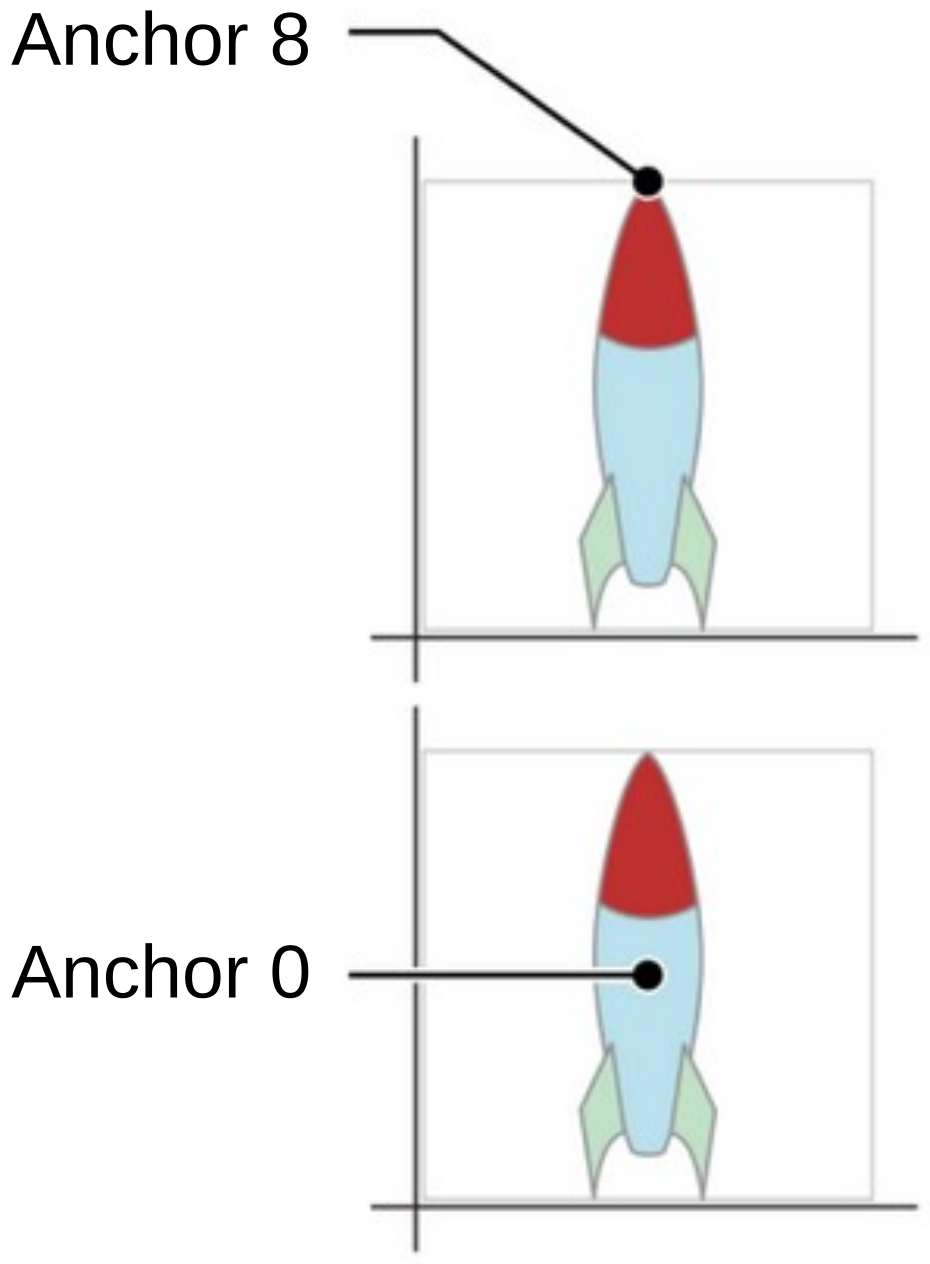
\includegraphics[width=0.25\textwidth]{neo6502-rocket.png}
\end{wrapfigure}
~\newline

To the right are two examples. Assume this is a 32x32 sprite.
In the upper example, the anchor point is at 8, the top-center.
Considering the origin at the bottom-left,
this sprite is drawn at 16,32, the midpoint of the top of the square.
% same as Q20: what is "the square"? - is this the bounding box of the sprite?
%              with respect to the origin,
%              both diagrams show the image drawn in exactly the same place
\newline

In the lower example, the anchor point is at 0;
and this sprite is drawn at 16,16 (the middle of the square).
The anchor point should be something like the centre point.
So for a walking character, this might be anchor point 2 (the bottom-center).
% same as Q20: "something like" is rather vague
%              rather "The anchor point should be ...":
%              "... thought of as the center point of" ... but of what? (eg: rotation?)
%              or:
%              "... placed near the center point of" ...but of what?
%              Anchor point 8 in the example image is not the center point of the image
%              nor is it the center point of the diagram.
%              The diagrams do not demonstrate anything that the table above does not
%              would this be better described as a "pivot point"?
%              Maybe the diagram of anchor point 8 should be re-centered about anchor point 8?
%              Maybe the rocket should be re-centered about anchor point 8?
%              Or is this the point which corresponds to the coordinates
%              WRT Function 6,2 "Sprite Set" and/or Function 6,2 "Sprite Get Position"?
%              Or is this related to collision detection?


\pagebreak


\section{Sound}\label{sound}

Function 8,4 queues a sound. Queued sounds are played sequentially,
each after the previous has completed,
such that sounds within a channel queue will not conflict, interrupt, or overlap.
\newline

Frequency is in units of Hertz.
Duration is in units of 100ths of a second.
Slide is a gradual linear change in frequency, in units of Hz per 100th of a second.
Sound source type 0 is the beeper.
Currently, the beeper is the only available sound source.
\newline

\ParamsBytes{Queue Sound Parameters}{Channel}{Freq hi}{Freq lo}{Duration lo}
                                    {Duration hi}{Slide lo}{Slide hi}{Source}



Function 8,5 plays a sound effect immediately. These will be synthesised to the best
ability of the available hardware. These are predefined as :

\begin{table}[h]
\begin{tabular}{ | c | c | }        \hline
\textbf{Number} & \textbf{Effect}   \\ \hline
\MonoSp{0} & positive \\ \hline
\MonoSp{1} & negative \\ \hline
\MonoSp{2} & error \\ \hline
\MonoSp{3} & confirm \\ \hline
\MonoSp{4} & reject \\ \hline
\MonoSp{5} & sweep \\ \hline
\MonoSp{6} & coin \\ \hline
\MonoSp{7} & las70 \\ \hline
\MonoSp{8} & powerup \\ \hline
\MonoSp{9} & victory \\ \hline
\MonoSp{10} & defeat \\ \hline
\MonoSp{11} & fanfare \\ \hline
\MonoSp{12} & alarm 1 \\ \hline
\MonoSp{13} & alarm 2 \\ \hline
\MonoSp{14} & alarm 3 \\ \hline
\MonoSp{15} & ringtone 1 \\ \hline
\MonoSp{16} & ringtone 2 \\ \hline
\MonoSp{17} & ringtone 3 \\ \hline
\MonoSp{18} & danger \\ \hline
\MonoSp{19} & expl100 \\ \hline
\MonoSp{20} & expl50 \\ \hline
\MonoSp{21} & expl20 \\ \hline
\MonoSp{22} & las30 \\ \hline
\MonoSp{23} & las10 \\ \hline
\end{tabular}
\end{table}

\end{document}
